
\chapter{Biomasa}
\label{chap:biomasa}
 
\section{Biomasa v kontextu energetiky}
\label{sec:biomasa-energetika}
 
Biomasa je z~historického hlediska nejstarším využívaným zdrojem energie. Dřevo jako základní palivo pro získávání tepelné energie dominovalo lidské energetice prakticky až do poloviny 18.~století, kdy jej začala postupně nahrazovat fosilní paliva, zejména uhlí. Ke konci 20.~století se však v~souvislosti s~rostoucím povědomím o~změně klimatu a~snahou o~snížení emisí skleníkových plynů vrátila biomasa opět do centra zájmu energetického sektoru. V~roce 2024 představovala biomasa (tuhá, kapalná i~plynná biopaliva) přibližně $46~\%$ celkové spotřeby obnovitelné energie v~Evropské 
unii \citep{eea_2025}, čímž si udržuje pozici největšího 
jednotlivého obnovitelného zdroje před větrnou ($18~\%$), vodní 
($12~\%$) a~solární energií ($11~\%$) \citep{eea_2025}. Celkový 
podíl obnovitelných zdrojů na~hrubé konečné spotřebě energie 
v~EU dosáhl v~roce 2024 hodnoty $25{,}2~\%$ \citep{eurostat_2025}.

Moderní bioenergie a biomasa si udržují zcela klíčové a nezastupitelné
postavení v globální energetické transformaci, a to zejména v sektorech,
které je obtížné dekarbonizovat. V oblasti elektroenergetiky vzrostla
v~roce 2024 globální kapacita zařízení pro výrobu elektřiny z~biomasy
o~4,6~GW na celkových 155~GW, přičemž tento růst byl tažen primárně
novými instalacemi v~Číně a Francii \citep{ren21_2025}. Celková
celosvětová výroba elektřiny ze zařízení na pevnou biomasu dosáhla
711~TWh.
 
Ještě podstatnější je však role biomasy v~sektoru vytápění a průmyslu.
Moderní bioenergie v~roce 2024 zajistila 8,3~\% celosvětové dodávky
tepla, přičemž pevná biomasa představuje hlavní zdroj pro sítě dálkového
vytápění \citep{ren21_2025}. V~průmyslovém sektoru je dominance biomasy
zcela zřejmá, neboť tvoří 89~\% veškerého spotřebovaného obnovitelného
tepla. Značný význam má také v~zemědělství, kde teplo tvoří téměř tři
čtvrtiny spotřebované energie; 10~\% tohoto tepla je obnovitelné
a~téměř výhradně pochází z~moderní bioenergie \citep{ren21_2025}. Celosystémový význam bioenergetiky podtrhuje také její silný
socioekonomický přínos, neboť v~roce 2023 tento sektor zaměstnával
3,9~milionu osob, čímž tvořil 24~\% veškeré pracovní síly v~obnovitelné
energetice a~byl druhým největším zaměstnavatelem v~tomto globálním
odvětví \citep{ren21_2025}.
 
Pojem biomasa lze v~energetickém kontextu definovat jako organickou hmotu rostlinného nebo živočišného původu, v~níž je prostřednictvím fotosyntézy uložena sluneční energie ve formě chemických vazeb a~která může být využita pro spalování či jiné přeměny s~následným energetickým využitím \citep{McKendry2002a}. 


 
Biomasu využitelnou pro energetické účely lze rozdělit do dvou základních kategorií. První kategorií je zbytková biomasa -- dřevní zbytky z~lesnictví (větve, kůra, pařezy), odpady dřevozpracujícího průmyslu (piliny, hobliny, odřezky), zbytky ze zemědělské výroby (sláma, zvířecí exkrementy) a~organické složky komunálního odpadu. Druhou kategorií je cíleně pěstovaná biomasa, tedy energetické plodiny a~rychle rostoucí dřeviny zakládané s~primárním cílem produkce biomasy pro energetické účely \citep{McKendry2002a}.
 
Z~hlediska způsobů energetického využití se biomasa zpracovává několika 
technologickými postupy. Nejrozšířenější metodou je přímé spalování, 
uplatňující se jak v~domácnostech (kotle na dřevo, pelety a~brikety), tak 
v~průmyslovém měřítku v~elektrárnách a~teplárnách. Účinnost využití biomasy závisí významně na~zvolené technologii. 
Při kombinované výrobě elektřiny a~tepla (kogeneraci) se celková 
účinnost (tepelná + elektrická) typicky pohybuje v~rozmezí 
$80$--$90~\%$ \citep{irena_2015,ctcn_2017}, což představuje 
nejvyšší celkovou účinnost využití energie z~biomasy. Moderní 
samostatné kotle na~biomasu (pelety, štěpka) v~teplárenství 
i~průmyslu dosahují tepelné účinnosti $85$--$90~\%$ 
\citep{roman_2024}. Při čisté výrobě elektřiny 
v~dedikovaných biomasových elektrárnách klesá elektrická 
účinnost na~$30$--$34~\%$ u~suché biomasy\citep{irena_2015}. Mezi další způsoby využití patří zplyňování, pyrolýza, anaerobní fermentace za vzniku bioplynu a~výroba kapalných biopaliv. V~kontextu biopaliv se rozlišují biopaliva první generace, vyráběná z~plodin konkurujících potravinářství (řepka, kukuřice), a~perspektivnější biopaliva druhé generace z~nepotravinářské biomasy. Směrnice Evropského parlamentu a~Rady EU/2023/2413 (tzv.~RED~III), která vstoupila v~platnost v~listopadu 2023, stanovuje závazný cíl podílu obnovitelných zdrojů minimálně 42{,}5\,\% do roku 2030 a~současně zpřísňuje kritéria udržitelnosti pro využívání biomasy \citep{REDIII2023}.
 
Významnou předností biomasy je její CO\textsubscript{2} neutrální charakter -- při spalování se uvolňuje prakticky stejné množství oxidu uhličitého, které bylo z~atmosféry odebráno během růstu rostliny. Navíc kořenový systém rostlin zadržuje přeměněný uhlík v~půdě podstatně déle, než je životnost nadzemní biomasy, což představuje mechanismus sekvestrace uhlíku. Například \citet{AduFosu2024} na základě desetiletého experimentu prokázali průměrnou rychlost sekvestrace uhlíku v~půdě pod porostem \textit{Miscanthus} na úrovni 0{,}83--1{,}37~Mg~C~ha\textsuperscript{-1}~rok\textsuperscript{-1}. Mezi další výhody patří lokální dostupnost zdroje, podpora venkovských oblastí, možnost využití přebytečné zemědělské půdy a~snížení závislosti na dovozech fosilních paliv. Na druhé straně je třeba zmínit omezení, jako je nízká energetická hustota ve srovnání s~fosilními palivy, vysoké přepravní náklady, nutnost úpravy paliva a~sezónnost dostupnosti některých zdrojů.
 
 
\section{Cíleně pěstovaná biomasa: \textit{Miscanthus} a~rychle rostoucí dřeviny (RRD)}
\label{sec:cilene-pestovana-biomasa}

V~podmínkách střední Evropy se pro cílené pěstování biomasy pro energetické účely etablovaly především dvě skupiny plodin: vytrvalé energetické trávy, reprezentované zejména ozdobnicí obrovskou (\textit{Miscanthus $\times$ giganteus}), a~rychle rostoucí dřeviny (RRD) pěstované ve výmladkových plantážích (\textit{Short Rotation Coppice}, SRC), zejména vrby (rod \textit{Salix}) a~topoly (rod \textit{Populus}). Tyto plodiny se vyznačují odlišnou agrotechnikou, dynamikou výnosů, strukturou peněžních toků a~rizikovým profilem, což je činí vhodnými pro komparativní analýzu a~potenciální diverzifikaci zemědělské produkce.

V~následujících kapitolách jsou všechny výnosy biomasy uváděny jako
\emph{suchá hmota} (zkratka~\textbf{DM}, z~angl.~\textit{dry matter}), tedy
biomasa po~odečtení obsahu vody (vlhkost $w = 0~\%$). Pokud není v~textu
uvedeno jinak (např.~„mokrá hmota při sklizňové vlhkosti"), všechny
hodnoty v~jednotkách t~DM/ha či~EUR/t~DM odkazují na~tuto sušinovou bázi.
Tato volba zajišťuje konzistentní srovnatelnost výnosů napříč plodinami
a~klimatickými zónami, neboť eliminuje rozptyl daný rozdílnou vlhkostí
biomasy v~okamžiku sklizně.

\subsection{Ozdobnice (\textit{Miscanthus})}
\label{subsec:miscanthus}

Rod \textit{Miscanthus} zahrnuje vytrvalé oddenkové trávy z~čeledi lipnicovitých (\textit{Poaceae}), původem z~východní Asie. Pro energetické účely je nejvýznamnější triploidní hybrid \textit{Miscanthus $\times$ giganteus}, který vznikl křížením \textit{M.~sinensis} a~\textit{M.~sacchariflorus}. Tato rostlina dosahuje výšky až 4~metry a~vykazuje řadu agronomických a~energetických předností \citep{Lewandowski2003}.

\textit{Miscanthus} je rostlinou s~C\textsubscript{4} fotosyntézou, což jí umožňuje efektivnější využití slunečního záření, vody a~živin ve srovnání s~C\textsubscript{3} rostlinami, které dominují v~mírném pásu. Spolu s~kukuřicí je jednou z~mála hospodářsky významných C\textsubscript{4} plodin adaptovaných na chladnější klima střední Evropy. Mezi její klíčové vlastnosti patří vysoká adaptabilita na různé půdní a~klimatické podmínky, schopnost růstu na méně úrodných půdách, vysoké výnosy sušiny, vysoká výhřevnost, odolnost vůči chorobám a~škůdcům a~nízké nároky na vstupy \citep{Lewandowski2003}.

Průměrné výnosy sušiny \textit{Miscanthus~$\times$~giganteus} jsou silně 
závislé na klimatické zóně, kvalitě půdy a~dostupnosti vody. 
\citet{mccalmont_2017} na základě přehledu devíti evropských sledovacích 
studií uvádějí typický rozsah ročních výnosů 10--15~t~DM/ha, přičemž 
na marginální zemědělské půdě (UK ALC grade 3b--5) modelovaný průměrný 
výnos činí přibližně 10~t~DM/ha. Konkrétní hodnoty z~evropských lokalit 
se pohybují v~rozsahu 8,75--16~t~DM/ha v~závislosti na klimatu, půdě 
a~věku porostu. V~podmínkách České republiky se na optimálních půdách výnosy pohybují 
v~rozmezí 14--16~t~DM/ha, na průměrných půdách 7--14~t~DM/ha 
a~na marginálních půdách klesají na 4--7~t~DM/ha \citep{VUKOZ2026}. 

Podle \citet{ThetaMetodika2024} se v~českých modelech počítá s~výhřevností
13{,}75~GJ/t při 20\,\% vlhkosti, což odpovídá vlhkosti biomasy
v~okamžiku zimní/jarní sklizně po~přirozeném proschnutí na~poli;
v~přepočtu na~suchou hmotu (DM, $w = 0\,\%$) činí výhřevnost
17{,}61~GJ/t~DM.

Agrotechnicky se ozdobnice množí vegetativně oddenky (rhizomy), jelikož v~mírném pásu nedochází k~dozrávání semen. Jako sterilní hybrid nevykazuje invazivní potenciál. Porost se zakládá jednorázově a~poskytuje roční sklizeň po dobu typicky 20--25~let. Výnosová dynamika je sigmoidální: plného potenciálu dosahuje plodina ve 3.--4.~roce, následuje stabilní období a~postupný pokles. Sklizeň probíhá v~předjarním období (únor--duben).

Environmentální přínosy pěstování ozdobnice jsou značné. \citet{mccalmont_2017} uvádějí, že energetický poměr (výstup/vstup) je u~\textit{Miscanthus} přibližně desetkrát vyšší než u~jednoletých energetických plodin a~uhlíkové náklady na výrobu energie jsou 20--30krát nižší než u~fosilních paliv. Pěstování ozdobnice na orné půdě zvyšuje obsah organického uhlíku v~půdě (sekvestrace 0{,}7--2{,}2~Mg~C\textsubscript{4}-C~ha\textsuperscript{-1}~rok\textsuperscript{-1})\citep{mccalmont_2017}.

Z~ekonomického hlediska představuje největší počáteční nákladovou položku
pořízení sadby. Z~kombinace dvou tržních zdrojů~--- lokálního českého
dodavatele za~0{,}50~EUR/kus \citep{Trogl2026} a~průměrné nabídky
evropských producentů v~rozsahu 0{,}16--0{,}21~EUR/kus
\citep{MiscanthusEU2026}~--- volíme kompromisní cenu 0{,}30~EUR/kus
zahrnující dopravu a~manipulační rezervu. Při doporučené hustotě výsadby
8\,000~oddenků/ha \citep{Weger2021} činí celkové investiční náklady
(CAPEX) přibližně 3\,045~EUR/ha. Roční provozní náklady ve~fázi
produkce dosahují přibližně 100~EUR/ha \citep{Wagner2022}. Výchozí
prodejní cena 117~EUR/t~DM je odvozena z~referenčního měrného nákladu
paliva 190~Kč/GJ \citep{ERU2025VymerBiomasa}; volatilita ceny činí
přibližně 20~EUR/t~DM. Riziko neúspěšného založení v~prvním roce je
odhadováno na~5~\% \citep{VUKOZ2026}. Detailní metodologie nákladů
a~ceny je uvedena v~sekci~\ref{sec:cenovy_model}.

\begin{figure}[H]
  \centering
  \includegraphics[width=1\textwidth]{cs/img/miscanthus_plantation.jpg}
  \caption[Plantáž \textit{Miscanthus $\times$ giganteus}]
  {Plantáž \textit{Miscanthus $\times$ giganteus} v~Kaneně 
  (Sasko-Anhaltsko, Německo). Foto: Katrin Schneider, 
  \href{http://korina.info}{korina.info}, Wikimedia Commons, 
  licence CC~BY-SA~4.0.}
  \label{fig:miscanthus-plantation}
\end{figure}

\subsection{Rychle rostoucí dřeviny (RRD) }
\label{subsec:src}

Rychle rostoucí dřeviny (RRD) pěstované ve výmladkových plantážích
(\textit{Short Rotation Coppice}, SRC) představují další významnou
skupinu pro produkci tuhé dřevní biomasy. Tyto plantáže jsou sklízeny
v~krátkých obmýtích (3--5 let) a~mají schopnost opakované regenerace
bez nutnosti nové výsadby. Výnosy vrb ve~střední Evropě závisejí
silně na~kvalitě půdy: na~optimálních půdách dosahují
12--15~t~DM/ha/rok, na~průměrných půdách 7--12~t~DM/ha/rok,
na~neúrodných půdách 4--7~t~DM/ha/rok a~na~nevhodných půdách
klesají na~0--4~t~DM/ha/rok (dle konzultací s~VÚKOZ Průhonice). Tyto
hodnoty jsou v~souladu s~typickým rozsahem výnosů SRC vrbových plantáží
v~Evropě, který se obvykle pohybuje mezi 5--18~t~DM/ha/rok v~závislosti
na~klimatické zóně a~bonitě půdy \citep{dimitriou_2015}.Přehledová studie \citet{Rodrigues2021} uvádí průměrnou produktivitu
RRD \textbf{12--14~t~DM/ha/rok} s~výhřevností sušiny
\textbf{16--19~GJ/t~DM}, životností 20--30~let a~potenciálem redukce
emisí skleníkových plynů o~90--99\,\% oproti
uhelným elektrárnám. \citet{ThetaMetodika2024} uvádí pro SRC výhřevnost
sušiny \textbf{18{,}39~GJ/t~DM} (při 0\,\% vlhkosti).

V~Evropě dominují v~SRC plantážích vrby (rod \textit{Salix}) a~topoly 
(rod \textit{Populus}). Vrby jsou preferovány 
pro svou toleranci k~širokému rozsahu půd, schopnost regenerace po sklizni 
a~odolnost kořenového systému vůči anoxickým podmínkám, což umožňuje jejich 
pěstování i~na zamokřených stanovištích \citep{dimitriou_2015}.

Zásadní rozdíl oproti ozdobnici spočívá ve struktuře peněžních toků. Zatímco \textit{Miscanthus} generuje roční příjmy, RRD akumulují biomasu po dobu 3--5 let a~příjmy ze sklizně jsou realizovány jednorázově na konci každého cyklu. Mezi sklizněmi plantáž generuje pouze náklady na údržbu, což zvyšuje nároky na finanční plánování a~řízení likvidity pěstitele.



Hlavním využitím biomasy z~RRD je lokální a~regionální bioenergetika, kde se dřevní štěpka spaluje pro výrobu tepla nebo v~kogeneračních jednotkách. SRC plantáže mají multifunkční charakter, plní ekosystémové funkce a~jejich životnost je obvykle 20--30 let, po které lze pozemek vrátit do původního stavu.

Sadební materiál v~podobě řízků vrby je výrazně levnější než oddenky
Miscanthus: při ceně 0{,}12~EUR/kus a~doporučené hustotě 7\,000~ks/ha
\citep{VUKOZ2026} činí celkové investiční náklady přibližně 1\,509~EUR/ha.
Roční provozní náklady na~údržbu jsou u~dobře založené plantáže
minimální, přibližně 50~EUR/ha/rok \citep{VUKOZ2026}. Sklizeň probíhá
v~tříletém cyklu s~náklady cca 40~EUR/t. Likvidace plantáže na~konci
životnosti je oproti Miscanthusu náročnější (cca 620~EUR/ha) kvůli nutnosti
dvouletého biologicko-mechanického rušení pařezů. Výchozí prodejní
cena 130~EUR/t DM je odvozena z~referenčního nákladu ERÚ; empirická
volatilita této ceny činí přibližně 16,6~EUR/t \citep{CSU2025LesnictviI}.
Detailní metodologie v~sekci~\ref{sec:cenovy_model}.
\begin{figure}[H]
  \centering
  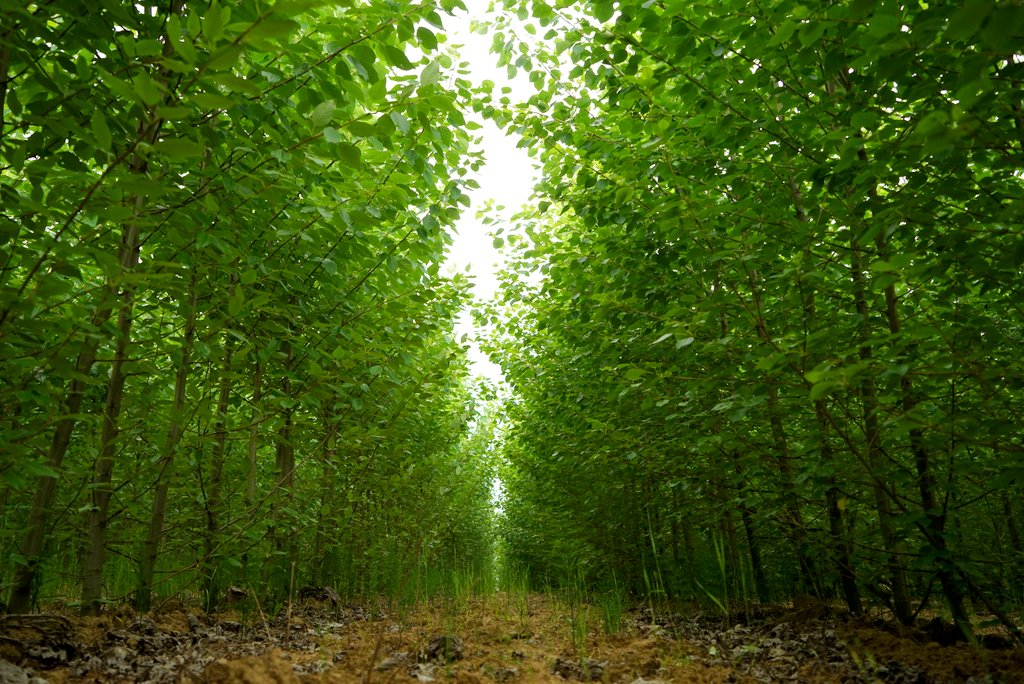
\includegraphics[width=0.9\textwidth]{cs/img/src_plantation.jpg}
  \caption[Výmladková plantáž rychle rostoucích dřevin (SRC)]
  {Dvouletá výmladková plantáž rychle rostoucích dřevin (SRC) 
  topolu (\textit{Populus} sp.) v~Brandenbursku (Německo). 
  V~podmínkách střední Evropy se v~SRC plantážích uplatňují 
  jak topoly, tak vrby (\textit{Salix}~sp.), které mají 
  obdobné agronomické a~ekonomické charakteristiky. 
  Foto: Lignovis GmbH, Wikimedia Commons, licence 
  CC~BY-SA~4.0.}
  \label{fig:src-plantation}
\end{figure}

\subsection{Srovnání a~motivace pro stochastické modelování}
\label{subsec:srovnani}

Tabulka~\ref{tab:srovnani_biomasy} shrnuje klíčové parametry obou plodin, které jsou relevantní pro ekonomické a~energetické hodnocení. Přestože se jedná o~zjednodušený přehled, ilustruje zásadní rozdíly v~charakteru produkce, které mají přímý dopad na volbu modelovacího přístupu.

\begin{table}[H]
    \centering
    \small
    \renewcommand{\arraystretch}{1.5}
    \caption{Srovnání \textit{Miscanthus} a~RRD vrb}
    \label{tab:srovnani_biomasy}
    \begin{tabularx}{\textwidth}{|>{\raggedright\arraybackslash}m{3.2cm}|>{\centering\arraybackslash}X|>{\centering\arraybackslash}X|}
        \hline
        \centering\textbf{Parametr} & \textbf{\textit{Miscanthus} $\times$ giganteus} & \textbf{RRD vrby (\textit{Salix})} \\
        \hline
        \textbf{Typ plodiny} & Vytrvalá tráva C\textsubscript{4} & Listnatá dřevina \\
        \hline
        \textbf{Životnost plantáže} & 20--25 let & 20--30 let (rotace) \\
        \hline
        \textbf{Množení} & Oddenky (vegetativně) & Řízky (vegetativně) \\
        \hline
        \textbf{Výnosová dynamika} & Sigmoidální; plný výnos ve 3.--4.~roce, roční sklizeň & Cyklická; sklizeň každé 3--5 roky, efekt učení \\
        \hline
        \textbf{Výnos (t~sušiny/ha/rok)} & 14--16 (stř. Evropa, opt. půda) & 12--15 (stř. Evropa, opt. půda) \\
        \hline
        \textbf{Výhřevnost (MJ/kg)} & $\approx$17 (při 5\,\% vlhkosti) & 16--19 (suchá hmota) \\
        \hline
        \textbf{Peněžní toky} & Roční příjmy ze sklizně & Příjmy jednorázově po každém cyklu \\
        \hline
        \textbf{Invazivní potenciál} & Nízký (sterilní hybrid) & Nízký (řízená kultivace) \\
        \hline
        \textbf{Enviro. přínosy} & Sekvestrace C, fytoremediace & Protierozní ochrana, biodiverzita, sekvestrace C \\
        \hline
        \textbf{Investiční náklady}     & $\approx$~3\,045~EUR/ha           & $\approx$~1\,509~EUR/ha          \\
        \hline
\textbf{Prodejní cena}    & $\approx$~117~EUR/t~DM  & $\approx$~130~EUR/t~DM  \\
\hline
        \textbf{Hlavní rizika} & Produkční, cenové & Produkční, cenové, likviditní \\
        \hline
    \end{tabularx}
\end{table}


Z~tabulky je patrné, že obě plodiny sdílejí řadu společných rysů -- jsou to vytrvalé energetické plodiny s~dlouhodobým horizontem investice, nízkou potřebou vstupů po fázi etablování a~významnými environmentálními přínosy. Současně se však zásadně liší ve výnosové dynamice, struktuře peněžních toků a~profilu rizik, což má přímé důsledky pro ekonomické modelování.

Deterministické modely pracující s~fixními hodnotami vstupních parametrů 
nemohou adekvátně zachytit inherentní nejistotu spojenou s~pěstováním 
energetických plodin. Výnosy \textit{Miscanthus} i~SRC vrb vykazují 
značnou meziroční variabilitu způsobenou klimatickými podmínkami --- 
zejména rozložením srážek během vegetačního období, výskytem pozdních 
mrazíků a~délkou bezfrostového období \citep{CliftonBrown2024}.

Variabilita ročních výnosů \textit{Miscanthus} v~podmínkách
České republiky je odhadována přibližně na~15~\%, zatímco u~SRC
vrb dosahuje pouze cca 10~\% \citep{knapek_2024}. Nižší
variabilita u~SRC je přičítána robustnějšímu kořenovému
systému dřevin, který tlumí vliv krátkodobých klimatických
výkyvů ve~srovnání s~trvalkami typu \textit{Miscanthus}.

Dalším klíčovým zdrojem nejistoty jsou tržní ceny biomasy a~energií.
Stanovení reprezentativní výkupní ceny je v~podmínkách České republiky
obtížné, neboť trh s~cíleně pěstovanou energetickou biomasou je
úzký a~málo likvidní. Pro SRC vrbu existuje alespoň částečně
funkční trh navázaný na~ceny dřevní štěpky a~palivového dříví, zatímco
\textit{Miscanthus} se v~současnosti v~energetickém sektoru ČR spíše
testuje v~rámci pilotních projektů a~spoluspalování, převážná část
produkce přitom končí v~nepalivových aplikacích (zejména stelivo
pro hospodářská zvířata, mulčování a~stavební materiály). Cena dřevní
štěpky a~slámy navíc podléhá sezónním výkyvům, regionálním disparitám
v~nabídce a~poptávce a~celkovému vývoji cen fosilních paliv. Podle dat
Teplárenského sdružení ČR dosahovala meziroční změna cen tepla
z~biomasy v~letech 2023--2025 v~některých případech až 20~\%,
přičemž konkrétní teplárny v~ČR vykazovaly zdražení v~rozmezí
14--20~\% meziročně \citep{tscr_2024}.

Do~ekonomiky projektů se dále promítá značná nejistota ohledně 
budoucí podoby dotačních schémat a~regulatorních požadavků. 
Ministerstvo průmyslu a~obchodu sice na~přelomu let 2024 a~2025 
spustilo aukce pro provozní podporu obnovitelných zdrojů 
(s~celkovým instalovaným elektrickým výkonem 13{,}12~MWe pro KVET 
zdroje) a~výzvu z~evropských fondů s~alokací 500~milionů Kč 
na~podporu výroby energie z~biomasy \citep{oEnergetice2025_podpora}, 
zelený bonus pro biomasové teplárny ale začne být vyplácen 
postupně a~jeho čerpání u~většiny podpořených projektů se 
očekává až v~období 2028--2030 \citep{oEnergetice2025_podpora}. 
Pro investora pěstujícího energetickou biomasu to znamená 
významnou nejistotu jak ohledně tempa rozvoje poptávky 
ze~strany tepláren, tak ohledně dlouhodobé stability dotačního 
rámce a~výkupních cen energie.
\section{Aktuální situace v~české energetice}
\label{sec:ceska-energetika}
 
Český energetický mix dlouhodobě stojí na dvou hlavních pilířích~-- jaderné energii a uhlí. V roce 2025 vzrostla celková netto výroba elektřiny v~ČR (poprvé od roku 2021) o~2{,}6~TWh na konečných 71{,}4~TWh. Tento růst byl tažen primárně jadernými elektrárnami, které vyrobily 30{,}3~TWh elektrické energie a podílely se tak na celkové výrobě z~42{,}4~\% \citep{oEnergetice2025}.
 
Zásadním hybatelem současných změn je však postupný útlum uhelných elektráren, jejichž provoz přestává být ekonomicky rentabilní kvůli kombinaci vysokých cen emisních povolenek a rostoucí produkce elektřiny ze solárních a větrných elektráren. Přestože uhelné zdroje v~roce 2025 stále vyrobily necelých 24~TWh (cca 32{,}2~\% celkové výroby), představuje to oproti krizovému roku 2022 pokles o~28~\% \citep{oEnergetice2025}. Očekává se, že do roku 2028 klesne instalovaný výkon uhelných zdrojů v~ČR ze současných přibližně 7~GW na 4~GW, a po roce 2030 by se měl pohybovat pod hranicí 1~GW. Spotřeba elektřiny přitom v~roce 2025 mírně vzrostla o~2{,}3~\% na 59{,}3~TWh a do budoucna se predikuje její další růst vlivem elektrifikace dopravy a vytápění.
 
 
\subsection{Role obnovitelných zdrojů energie (OZE)}
 
Úbytek uhelných kapacit musí být kompenzován rozvojem obnovitelných zdrojů energie a plynových zdrojů. Z~hlediska podílu OZE na výrobě elektřiny Česká republika dlouhodobě zaostává za evropským průměrem a pravidelně se umisťuje mezi třemi státy EU s~nejnižším podílem zelené energie \citep{oEnergetice2025}.
 
Rok 2025 nicméně potvrdil postupně rostoucí roli OZE v~českém mixu. Celková výroba z~těchto zdrojů dosáhla zhruba 12{,}2~TWh, což odpovídá přibližně 17{,}1~\% celkové výroby elektřiny v~ČR. Vláda v~aktualizovaném Národním klimaticko-energetickém plánu vytyčila cíl dosáhnout 30~\% podílu OZE na hrubé konečné spotřebě energie do roku 2030 (oproti celounijnímu cíli 42{,}5~\%). Tento cíl odpovídá požadavkům směrnice RED~III \citep{REDIII2023}.
 
Z~pohledu struktury samotných obnovitelných zdrojů dominují v~ČR fotovoltaické elektrárny, které v~roce 2025 tvořily 38{,}9~\% veškeré zelené produkce. Hned na druhém místě se nachází \textbf{biomasa s~podílem 24{,}0~\%}, následovaná bioplynem (18{,}8~\%), vodními elektrárnami (13{,}4~\%) a větrnými elektrárnami (5{,}0~\%) \citep{oEnergetice2025}. Tento poměr je dlouhodobě stabilní, jak dokládá zpráva Ministerstva průmyslu a obchodu o~využívání OZE v~ČR \citep{MPO2024oze}.
 
\subsection{Instalovaný výkon a celkové postavení biomasy}
 
Zatímco solární a větrné elektrárny představují zdroje s~výrazně kolísavou výrobou závislou na počasí, biomasa tvoří stabilní a předvídatelný pilíř OZE. Ke konci roku 2025 bylo v~České republice evidováno 77 licencovaných provozoven spalujících biomasu, jejichž celkový instalovaný výkon činil přibližně 2{,}3~GW \citep{oEnergetice2025}. Specifikum biomasy spočívá v~jejím duálním využití~-- zatímco v~elektroenergetice plní spíše významnou doplňkovou roli, v~teplárenství je naprosto klíčovým nástrojem pro dekarbonizaci.
 
\subsection{Podíl na výrobě elektřiny}
 
V~roce 2025 dosáhla výroba elektrické energie z~biomasy objemu 2{,}9~TWh, což představuje podíl na celkové výrobě elektřiny v~ČR ve výši zhruba~4~\%. Nejdůležitějším fenoménem uplynulého roku byl však samotný růst produkce. Oproti roku 2024 zaznamenala výroba elektřiny z~biomasy mimořádně silný nárůst o~téměř 0{,}7~TWh, tedy o~30{,}7~\% \citep{oEnergetice2025}.
 
Tento výrazný růst je z~pohledu hodnocení potenciálu trhu velmi specifický. V~průběhu celého roku 2025 totiž nebyl pro výrobu elektřiny z~biomasy zprovozněn prakticky žádný nový instalovaný výkon, s~výjimkou jediné menší instalace Energoblok Blatno o~výkonu pouhých 175~kW. Skokový růst produkce tak dominantně pramenil z~mnohem vyššího využití stávajících zdrojů. Biomasa se technologicky využívá buď ve specializovaných teplárnách na biomasu, nebo dochází k~jejímu spoluspalování v~uhelných elektrárnách (přimíchávání dřevní štěpky k~uhlí), což provozovatelům pomáhá optimalizovat emisní zátěž \citep{oEnergetice2025}.
 
 
\subsection{Podíl na teplárenství}
 
Zatímco v~sektoru výroby elektřiny tvoří biomasa menší část národního mixu, v~českém teplárenství hraje naprosto stěžejní a dominantní roli. Z~aktuálních dat vyplývá, že téměř 90~\% veškeré produkce tepla z~obnovitelných zdrojů připadá právě na biomasu, což absolutně odpovídá přibližně 10\,000~TJ ročně \citep{oEnergetice2025}. Podle dat Energetického regulačního úřadu (ERÚ) představuje biomasa třetí nejvýznamnější zdroj dálkového tepla v~ČR celkově, po uhlí a zemním plynu, přičemž s~postupující dekarbonizací se její podíl dále zvyšuje \citep{FaktaOKlimatu2025}.
 
České teplárenství v~současnosti prochází dynamickou proměnou vynucenou rychlým odklonem od uhlí. Jen v~letech 2022 až 2024 ukončilo nebo výrazně omezilo spalování uhlí deset velkých tepláren. Tyto provozy nahradily přes 500~tisíc tun uhlí ročně palivy s~nižší emisní stopou~-- nejčastěji právě biomasou, případně zemním plynem. Díky těmto změnám došlo ke snížení emisí oxidu uhličitého o~více než 600~tisíc tun ročně \citep{oEnergetice2025}. Příkladem úspěšné konverze jsou teplárenské provozy v~Plané nad Lužnicí, Táboře či Kolíně, nebo teplárna ve Strakonicích, kde dnes biomasa pokrývá zhruba 98~\% spotřeby paliva.
 
Budoucí poptávku po cíleně pěstované biomase budou bezpochyby formovat další masivní investice. Očekává se, že celkové náklady na náhradu uhelných zdrojů v~českých teplárnách přesáhnou do konce tohoto desetiletí 200~miliard~Kč. Významnou ukázkou tohoto trendu je probíhající modernizace závodní teplárny ŠKO-ENERGO v~Mladé Boleslavi. Přestavba s~rozpočtem 4{,}5~miliardy~Kč byla zahájena v~září 2024 s~cílem přejít do roku 2027 na stoprocentní spalování biomasy \citep{oEnergetice2025}. Jak upozorňuje analýza projektu Fakta o~klimatu, právě kombinace biomasy se zemním plynem a tepelnými čerpadly představuje nejpravděpodobnější scénář dekarbonizace českého teplárenství v~horizontu do roku 2030 \citep{FaktaOKlimatu2025}.
 
Biomasa má své nezastupitelné uplatnění také v~malých zdrojích a domácnostech (kotle na pelety, kusové dřevo), a to zejména v~oblastech mimo dosah plynofikace. Podle zprávy MPO se pod pojmem biomasa v~národní energetické statistice rozumí veškeré palivové dříví, dřevní odpad i~produkty jako pelety a~brikety, přičemž spotřeba biomasy je sledována u~přibližně 30~tisíc subjektů \citep{MPO2024oze}. Nicméně i přes to, že absolutním těžištěm spotřeby biomasy jsou z hlediska vyrobeného tepla domácnosti, hraje biomasa z důvodu dekarbonizace stále významnější roli i ve větších zdrojích tepla a systémech centrálního zásobování teplem (CZT).
 
Rostoucí poptávka ze strany teplárenství a~energetiky vytváří přímou ekonomickou motivaci pro rozšiřování cíleného pěstování energetických plodin, ať už ozdobnice či výmladkových plantáží vrb. Současně však přináší otázku, zda je investice do takového pěstování pro zemědělce skutečně ekonomicky výhodná a~jaká rizika s~sebou nese. Kvantifikaci těchto rizik prostřednictvím stochastického simulačního modelu je věnována praktická část této práce.